When entereing an address in to any of the text fields, there are some limitations to what you can search for. It is possible to seach for any road name you want. An auto completions box pops up, while you are typing, giving you the possible cities where roads with the given name exist. It is also possible jus tto search for a city name or a zip code. If you wand to search for "\AA boulevarden" in Copenhagen, you will have to separete the search with a comma like "\AA boulevarden, K\o benhavn" and not "\AA boulevarden K\o benhavn". You will not be able to search for road numbers but only road names, so please have in mind that if a road is long, the map may not lead you to the exact desired point that you are searching for, but only the road that you are searching for.

To find a specific address on the map, all you need to do is to enter the address in the upper text field named "Point / from", and then press "Find". The address you have searched for will now be marked on the map with a little dot, and you will automatically be zoomed in to this point.

When you want to find a route from one point to another, you simply type in the address that you want to go from, in the "Point / from" field, and the address you want to go to in the "To" field. When you have entered the to desired addresses you press the "Find" button and the route will be drawn on the map with a pink color. 
It is also possible to swap the to address field, so that the "Point / from" address now becomes the "To" address and vice versa, by pressing the "Swap" button.

Under the "Swap" and "Find" buttons, two radio buttons are located. "Fast" and "Short". If the "Fast" button is chosen, which is standard, the fastest route between the two addresses will be found. This is useful for cars, since they are able to drive at different speed levels. If the "Short" button is chosen, the shortest route will be found. This is suitable if the user is walking, cycling or using any other relatively slow way to travel with a mostly constant speed. The standard speed for "Short" is 5 km/h, which means that the time the program calculates for your trip when using "Short", is only actual for travels by foot.

Under the two radio buttons there are two values shown. "Distance" and "Time". "Distance" shows the distance from the starting address to the endind address in kilometres. "Time" shows the estimated time that the trip will take. 

\begin{figure}[htb]
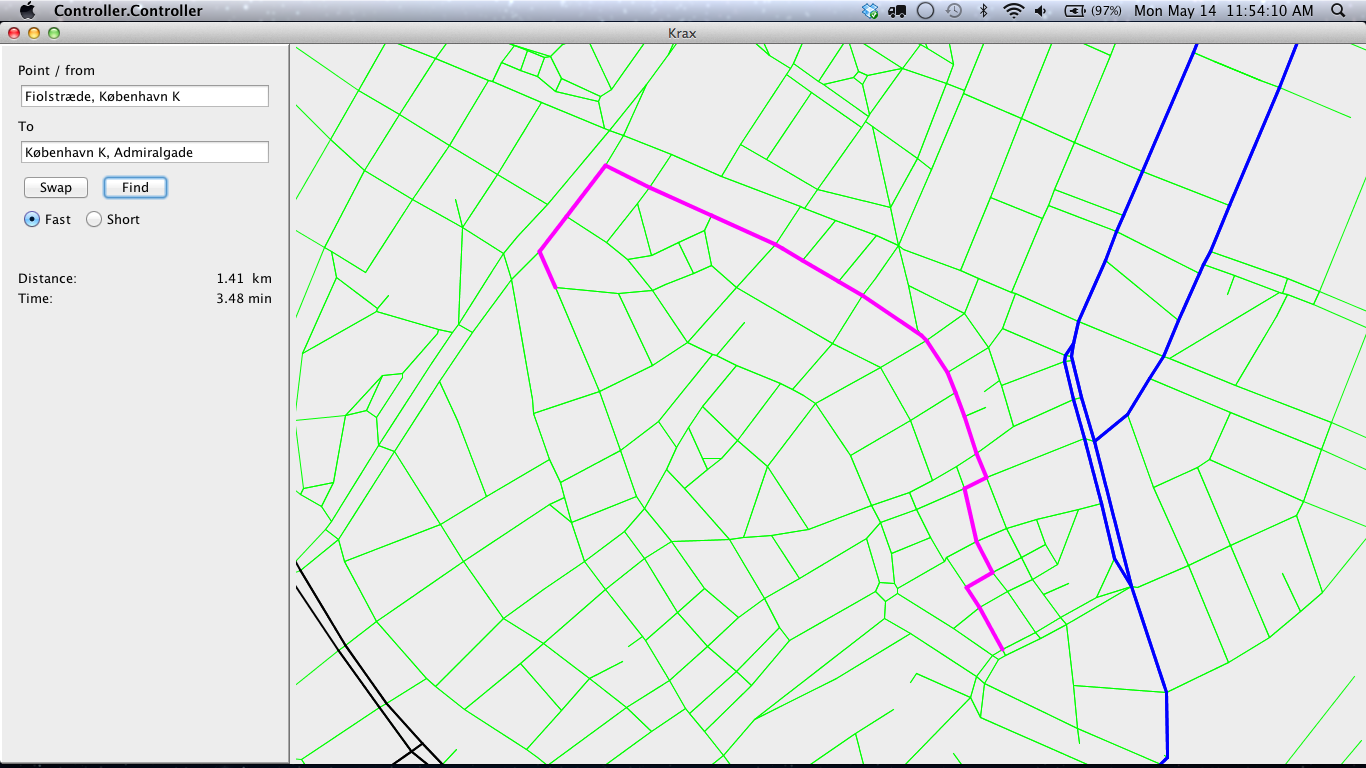
\includegraphics{User_manual/screenshot.png}
\end{figure}
